
\hypertarget{Analyse-et-traitement-des-donnuxe9es}{%}
\chapter{Analyse et traitement des données}\label{Analyse-et-traitement-des-donnuxe9es}}

Dans cette partie on va voir l'essentiel du travail que j'ai effectué durant mon stage à savoir la génération de fiches d'analyse de nos données. Dans un premier temps nous verrons les signaux, puis à l'aide d'un zoom les clics émis par les animaux. Ensuite afin d'affiner notre analyse nous verrons leurs transformées de Fourier grâce auxquelles nous obtiendrons leurs spectrogrammes 2D et 3D. Dans un second temps nous verrons l'une des principales méthodes de préparation des données que nous avons effectuée à savoir la \textit{data augmentation} d'abord d'un point de vue théorique puis d'un point de vue pratique avec la data augmentation que nous avons effectuée sur notre base à savoir le rajout de bruit blanc puis la simulation de distance. Dans un troisième temps nous verrons les prétraitements de données que nous avons dûs effectuer pour le bon fonctionnement de nos IA à savoir l'application d'un filtre passe haut puis une mise à l'échelle. Ensuite nous verrons les pipelines qui nous ont permis d'optimiser l'injection des flux de données dans nos réseaux de neurones. Et enfin nous verrons le résultat final regroupant ces différents éléments pour la génération des fiches d'analyse.

\hypertarget{Les-signaux}{%}
\section{Les signaux}
\label{Les-signaux}}
Les données sont fournies par les organisateurs du challenge sous la forme de tableaux d'échantillons. Chaque exemple, un son ou signal temporel correspondant à un clic, est ainsi composé de
8192 échantillons de l'amplitude sonore captée à une fréquence de 200KHz par un hydrophone.
Dans la suite du rapport, nous appelerons "signal" un exemple de la base d'apprentissage ou de test, pour conserver à l'esprit la nature des données que nous devons traiter.

Afin d'améliorer la lisibilité des sections suivantes nous prendrons comme fil rouge les trois mêmes signaux (le n°17000 et le n°20000 de la base labelisée ainsi que le n°571 de la base non labelisée).
Nous les avons choisis car ils sont représentatifs de la diversité des signaux que l'on a dans notre base à savoir :
\begin{itemize}
\item Des signaux très propres
\item Des signaux un peu bruités ou altérés
\item Des signaux très dégradés
\end{itemize}
Nous les observerons sous diverses formes puis nous effectuerons dessus un certain nombre de traitements.

\hypertarget{Signaux-Bruts}{%}
\subsection{Les signaux bruts}
\label{Signaux-Bruts}}

Dans un premier temps, nous commençons par observer les signaux sans traitement, comme des signaux sonores, c'est à dire comme l'évolution dans le temps de l'amplitude du son.

\begin{figure}[!h]
\centering
	\begin{subfigure}[b]{0.3\textwidth}
    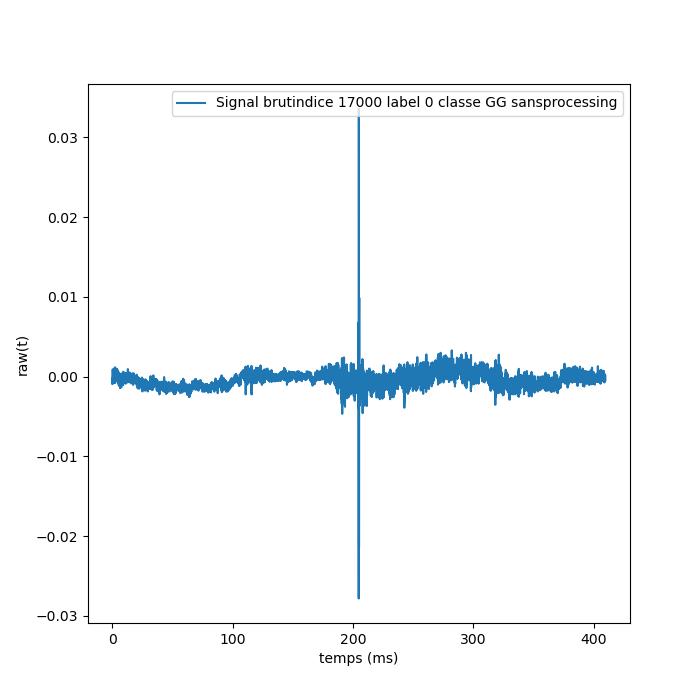
\includegraphics[width=\textwidth]{./images/indice17000Spectro1Dlabel0classeGGsansprocessingsanszoom.png}
    \caption{}
  	\end{subfigure}
  	\begin{subfigure}[b]{0.3\textwidth}
    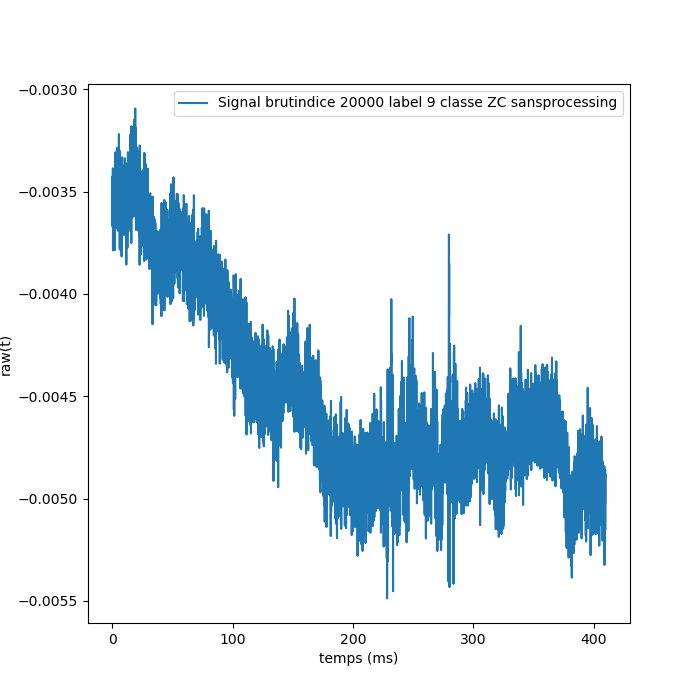
\includegraphics[width=\textwidth]{./images/indice20000Spectro1Dlabel9classeZCsansprocessingsanszoom.png}
	\caption{}
  	\end{subfigure}
  	\begin{subfigure}[b]{0.3\textwidth}
    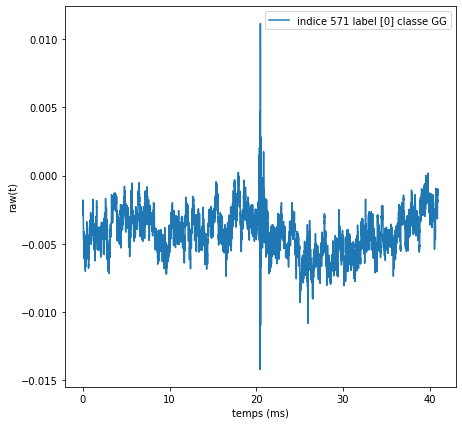
\includegraphics[width=\textwidth]{./images/indice571Spectro1Dlabel9classeZCsansprocessingsanszoom.png}
    	\caption{}
	\end{subfigure}
\caption{Signaux bruts : (a) n°17000 et (b) n°20000 de la base d'apprentissage ; (c) n°571 de la base de test.%
\label{fig:signauxbruts}}
\end{figure}

Sur la figure \ref{fig:signauxbruts}, nous constatons plusieurs choses : tout d'abord il semble y avoir une certaine disparité entre les signaux, certains étant beaucoup plus bruités que d'autres; de plus contrairement à ce que l'on pouvait penser, le clic n'est pas toujours facile à distinguer et celui-ci n'est pas non plus toujours bien centré.

Cependant, nous avons pu tirer quelques enseignements de l'observation de ces signaux :
\begin{itemize}
\item L'amplitude des clics semble variable : elle est de 0.06 pour le signal 17000 et de 0.020 pour le signal 571, par exemple.
\item Il arrive que le bruit soit suffisament important par rapport au clic pour rendre son identification difficile voir impossible, comme pour le signal 20000.
\end{itemize}

Pour afiner notre analyse, il parait pertinent de commencer par zoomer sur ce clic.
Pour cela il va donc faloir commencer par trouver un moyen d'isoler le clic.

\hypertarget{Le-zoom}{%}
\subsection{Le zoom}
\label{Le-zoom}}

Pour zoomer sur le clic, on identifie le maximum du signal qui sera, idéalement, le milieu du clic puis on rajoute l'équivalent de la durée d'un clic (qui est de l'ordre de 5 millisecondes) avant et aprés ce maximum.


\begin{figure}[!h]
  \centering
  \begin{subfigure}[b]{0.3\textwidth}
    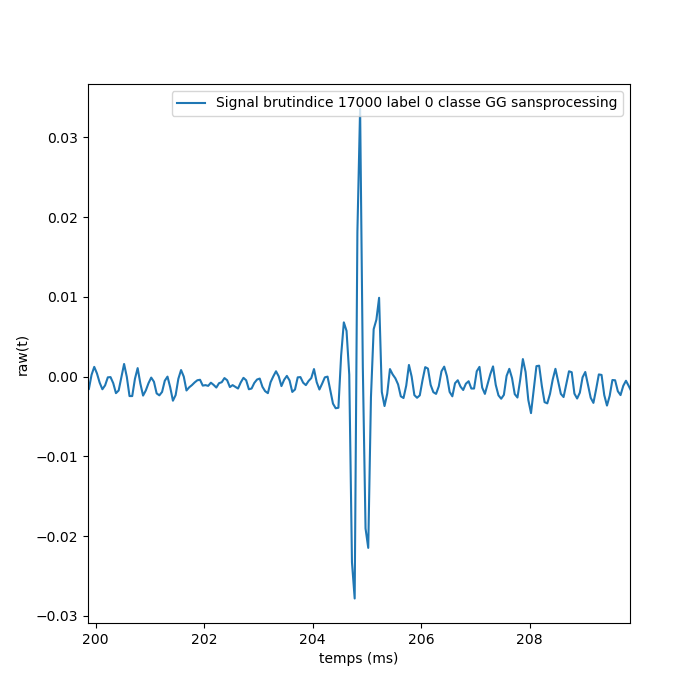
\includegraphics[width=\textwidth]{./images/indice17000Spectro1Dlabel0classeGGsansprocessingaveczoom.png}
    \caption{17000}
  \end{subfigure}
  \begin{subfigure}[b]{0.3\textwidth}
    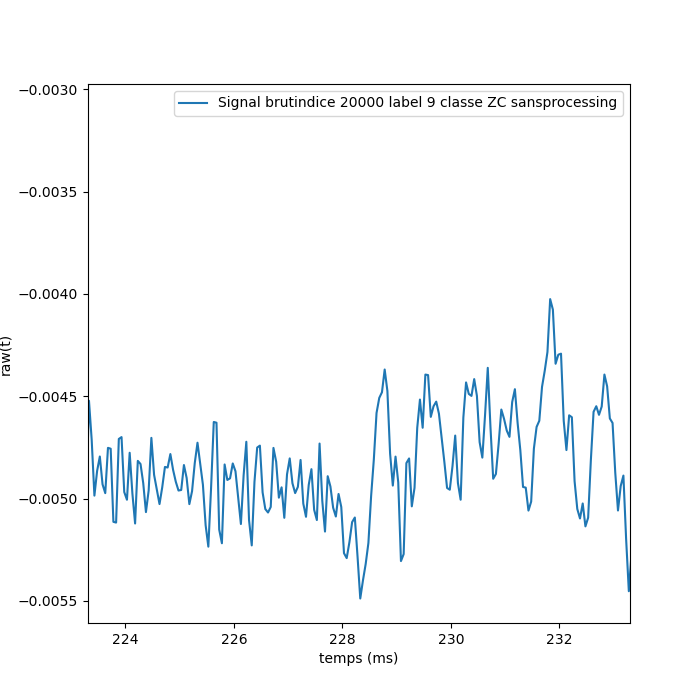
\includegraphics[width=\textwidth]{./images/indice20000Spectro1Dlabel9classeZCsansprocessingaveczoom.png}
  \caption{20000}
  \end{subfigure}
  \begin{subfigure}[b]{0.3\textwidth}
    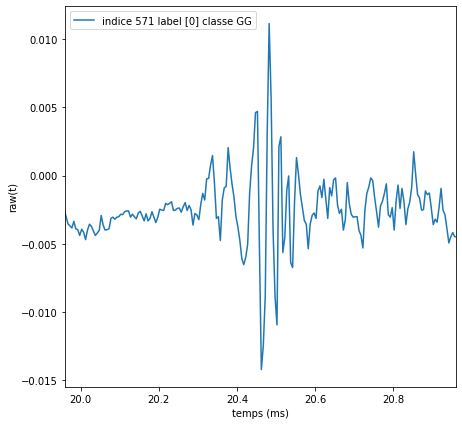
\includegraphics[width=\textwidth]{./images/indice571Spectro1Dlabel9classeZCsansprocessingaveczoom.png}
  \caption{571}
  \end{subfigure}
  \caption{Signaux bruts : (a) n°17000 et (b) n°20000 de la base d'apprentissage ; (c) n°571 de la base de test. avec un zoom temporel%
  \label{fig:signauxbrutszoom}}
\end{figure}

On peut observer le résultat de cette opération sur la figure~\ref{fig:signauxbrutszoom}.
Cela nous permet de constater que cette procédure n'est pas efficace dans tous les cas. En effet si pour les signaux n° 17 000 et 571 le zoom semble bien fonctionner dans le cas du signal n° 20 000 qui est très bruité, le bruit semble avoir pris le dessus sur le clic conduisant à l'echec de l'identification du clic.
On va donc par la suite appliquer un filtre pour supprimer une partie des bruits parasites (dont on reparlera dans la partie traitement du signal).

On peut déjà observer plusieurs phénoménes :
\begin{itemize}
\item L'efficacité du zoom semble corrélée à la qualité du signal de départ : un nettoyage du signal semble donc nécessaire pour améliorer la détection du clic.
\item L'intensité des clics est très  variable, cette variation pouvant aller jusqu'a un facteur 10 entre 2 clics : il parait donc pertinent par la suite de les normaliser.
\item La durée d'un clic est bien de l'ordre de 0.5 millisecondes.
\item Les clics les plus nets semblent bien centrés autour de 200 ms.
\end{itemize}

Sous cette forme, nos observations semblent quand même limitées.
Nous allons donc les observer sous d'autres formes puis on cherchera à améliorer la qualité de nos signaux via diverses techniques. Etant donné la nature de nos données à savoir des enregistrements audios, observer leurs spectrogrammes semble être pertinent.

\hypertarget{Transformuxe9-de-Fourier}{%}
\subsection{Transformée de Fourier}
\label{Transformuxe9-de-Fourier}}

Avant d'observer les spectrogrammes il convient de commencer par expliquer et observer les spectres obtenus par la transformée de Fourier de nos 3 signaux.

La transformée de Fourier est un outil mathématique nous permettant de passer du domaine temporel au domaine fréquenciel, en décomposant le signal de départ en somme de signaux sinusoidaux.
Cela permet d'observer les différentes composantes fréquentielles du signal.

Les transformées de Fourier de nos signaux sont présentées sur la figure~\ref{fig:tf} (les courbes ne sont pas du tout à la même échelle en ordonnée).
\begin{figure}[!h]
\centering
  \begin{subfigure}[b]{0.3\textwidth}
    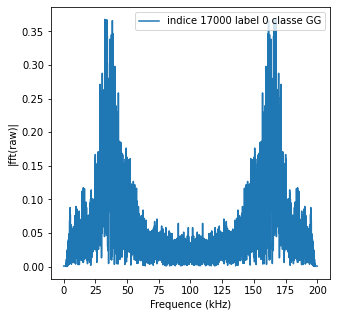
\includegraphics[width=\textwidth]{./images/17000fft.png}
  \end{subfigure}
  \begin{subfigure}[b]{0.3\textwidth}
    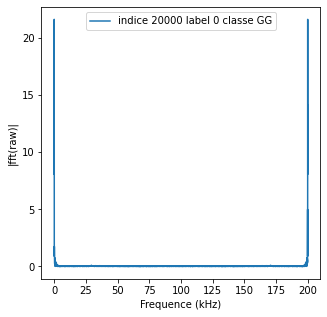
\includegraphics[width=\textwidth]{./images/20000fft.png}
  \end{subfigure}
  \begin{subfigure}[b]{0.3\textwidth}
    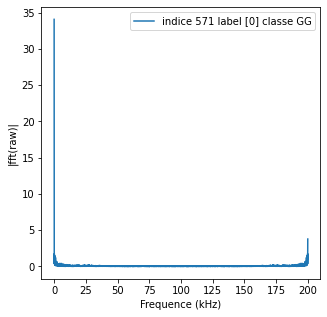
\includegraphics[width=\textwidth]{./images/571fft.png}
  \end{subfigure}
  \caption{Transformé de Fourier des signaux : (a) n°17000 et (b) n°20000 de la base d'apprentissage ; (c) n°571 de la base de test.%
\label{fig:tf}}
\end{figure}

Sur la figure \ref{fig:tf} on constate particuliérement sur le signal n° 17000 un pic entre les fréquence 25KHz et 50KHz, dont on peut supposer qu'il correspond au clic.
Par contre, les autres spectres, tels qu'ils sont représentés, avec des pics importants aux très basses fréquences, ne permettent pas de trouver le clic.

\hypertarget{Spectrogrammes}{%}
\subsection{Spectrogrammes}
\label{Spectrogrammes}}

Les spectrogrammes sont simplement des transformées de Fourier effectuées à chaque pas de temps, sur une fenêtre temporelle. Cela permet de visualiser l'évolution des fréquences au cours du temps.

On commence par observer, sur la figure~\ref{fig:spectros2D}, les spectrogrammes en 2D, avec l'amplitude qui est représentée par une échelle de couleur (a noter qu'ici pour éviter les phénoménes d'écrasement, les fréquences majoritaires pouvant écraser les autres, on utilise une échelle logarithmique pour les amplitudes).

\begin{figure}[!h]
  \centering
  \begin{subfigure}[b]{0.3\textwidth}
    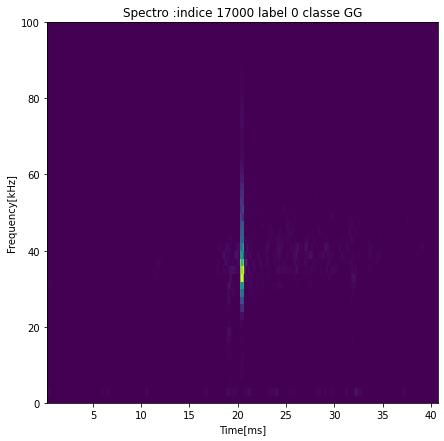
\includegraphics[width=\textwidth]{./images/indice17000Spectro2Dlabel0classeGGsansprocessingsanszoom.png}
    \caption{}
  \end{subfigure}
  \begin{subfigure}[b]{0.3\textwidth}
    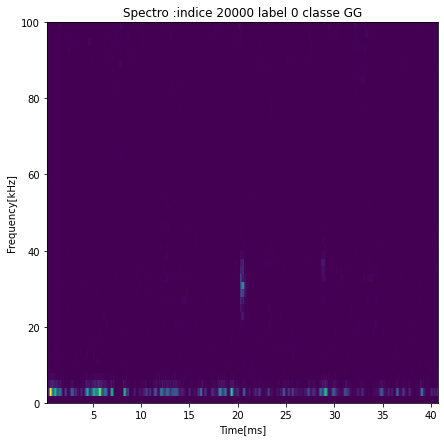
\includegraphics[width=\textwidth]{./images/indice20000Spectro2Dlabel9classeZCsansprocessingsanszoom.png}
    \caption{}
  \end{subfigure}
  \begin{subfigure}[b]{0.3\textwidth}
    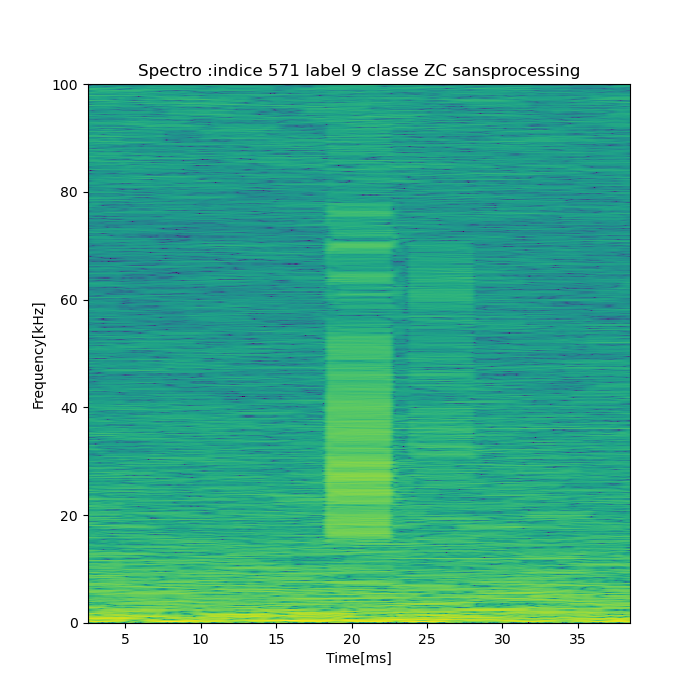
\includegraphics[width=\textwidth]{./images/indice571Spectro2Dlabel9classeZCsansprocessingsanszoom.png}
    \caption{}
  \end{subfigure}
  \caption{Spectrogramme 2D des signaux : (a) n°17000 et (b) n°20000 de la base d'apprentissage ; (c) n°571 de la base de test.%
  \label{fig:spectros2D}}
\end{figure}

On constate tout d'abord  que leurs gammes de fréquences semblent relativement variable d'un enregistrement à l'autre et que la visibilité des clics semble bien correlée à leur qualité.
Ainsi, pour le signal n° 17000 qui est de bonne qualité, le clic est très clairement visible : la bande verticale au centre de la figure de couleur vive.
Pour le signal n° 571 qui est peu dégradé le clic est encore assez visible.
A l'inverse, pour le signal n° 20000 qui est le plus dégradé, le clic est très peu visibleet plutôt sur les basses fréquences.

On constate également, ce qui n'apparaisait ni sur les signaux temporels ni sur les spectres que le clic principale sempble accompagné de répliques, ce qui est cohérent avec la biologie : il y a un phénomène d'écho à l'intérieur du nez des odontocètes lors de l'émission des clics.

On peut aussi visualiser les spectrogrammes en 3D, comme le montre la figure~\ref{fig:spectros3D}.
Les informations sont les mêmes, mais représentées différemment.
Cela permet d'avoir une meilleure idée de l'importance relative des pics de fréquence.
De plus, un intérêt qui n'est pas évident sur un affichage statique, cette visualisation en 3D permet de faire varier l'angle de vue, ce qui permet d'avoir des points de vue différents sur les courbes.

\begin{figure}[!h]
  \centering
  \begin{subfigure}[l]{0.5\textwidth}
    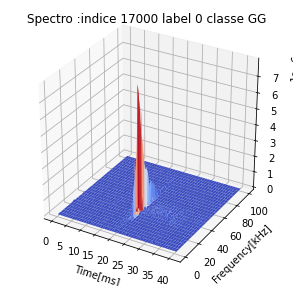
\includegraphics[width=\textwidth]{./images/indice17000Spectro3Dlabel0classeGGsansprocessingsanszoom.png}
        \caption{}
  \end{subfigure}
  \newline
  \begin{subfigure}[l]{0.5\textwidth}
    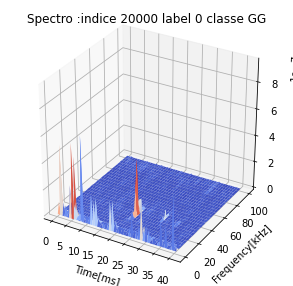
\includegraphics[width=\textwidth]{./images/indice20000Spectro3Dlabel9classeZCsansprocessingsanszoom.png}
        \caption{}
  \end{subfigure}
  \newline
  \begin{subfigure}[l]{0.5\textwidth}
    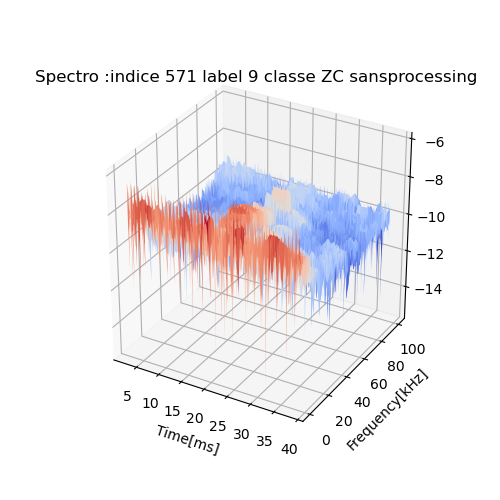
\includegraphics[width=\textwidth]{./images/indice571Spectro3Dlabel9classeZCsansprocessingsanszoom.png}
        \caption{}
  \end{subfigure}
  \newline
  \caption{Spectrogramme 3D des signaux : (a) n°17000 et (b) n°20000 de la base d'apprentissage ; (c) n°571 de la base de test.%
	\label{fig:spectros3D}}
\end{figure}

On constate bien mieux l'impact du bruit sur \ref{fig:spectros3D} les spectrogrammes 3D que sur les spectrogrammes 2D.

\hypertarget{Data-augmentation}
\subsection{Intérêt théorique}
\label{interets_theoriques}}

Basiquement, l'augmentation de données, ou data augmentation, regroupe un ensemble de méthodes permettant d'augmenter "artificiellement" la taille de la base sur laquelle le réseau de neurones va apprendre. Ainsi en plus de nos exemples initiaux on viendra rajouter de nouveaux exemples qui seront des versions "modifiées" des exemples initiaux.

Pour cela selon la nature des données de cette base on va par exemple :
\begin{itemize}
\item Flouter les exemples s'il s'agit d'images
\item Effectuer une rotation sur les exemples
\item Modifier la luminosité dans le cas d'images
\end{itemize}

Dans notre cas, dans la mesure où nos données sont des enregistrements audios, nous allons plutôt :
\begin{itemize}
\item Rajouter du bruit sur les exemples
\item Déplacer le clic
\item Simuler une modification de la distance entre l'animal et l'hydrophone
\end{itemize}

Nous avons décidé de ne pas inclure l'effet Doppler (modification des fréquence en fonction des vitesses relatives) dans la data augmentation, qui semble être
marginal.

L'intérêt le plus évident de cette opération est de multiplier le nombre d'exemples disponibles afin d'éviter le surapprentissage mais elle peut avoir beaucoup plus d'utilité.
En effet dans notre cas, nous n'avons rencontré aucun probléme de surapprentissage mais nous avons besoin de l'utiliser pour une autre raison.
Nous avons pu remarquer que certains exemples avaient subi de fortes dégradations notamment dues
à du bruit ou bien à un fort décalage temporel du clic par exemple.
Afin d'éviter que ces dégradations n'altérent le processus d'apprentissage de nos réseaux de neurones (le réseau pouvant par exemple assimiler une de ces dégradations à l'une des classes),
plutôt que de les supprimer, il nous a paru plus pertinent d'essayer de rajouter aléatoirement ces
pertubations sur tous les exemples.


\hypertarget{Rajout-de-bruit-blanc}{%}
\subsection{Rajout de bruit blanc}
\label{Rajout-de-bruit-blanc}}

Comme on a pu l'observer précedement certains enregistrement sont plus ou moins bruités.
Nous allons donc dans un premier temps essayer d'en diminuer l'impact via de la data augmentation. Autrement dit nous allons artificiellement créer des exemples issus d'enregistrements choisis aléatoirement auxquels du bruit a été artificiellement ajouté.
Le type de bruit que nous avons choisi, en dehors de toute indications sur les bruits marins, est un bruit blanc ou gaussien : au signal temporel est ajouté une valeur aléatoire de densité normale (moyenne 0, écart-type variable).

\hypertarget{Simulation-de-distance}{%}
\subsection{Simulation de distance}
\label{Simulation-de-distance}}

Lors de la prise des enregistrements audio les animaux peuvent se situer plus ou moins loin du ou des micro, ce qui peut potentiellement influencer notre classifieur.
En effet certaines espèces plus fuyardes peuvent par exemple rester systématiquement plus
éloignées du micro que les autres poussant le classifeur à assimiler
une grande distance à une espèce en particulier.
Afin d'éviter ce biais nous avons décidé de rajouter la simulation de distance dans la data augmentation.
Le principe est simple on va rajouter aléatoirement des signaux choisis dans des classes aléatoires à une distance aléatoire (on simule les effets de la distance sur le signal).
L'effet de la distance dans un milieu liquide est approximé une atténuation exponentielle des hautes fréquence.
Pour simuler cette atténuation, nous nous sommes basés sur des études en hydro-accoustique.

\hypertarget{Traitement-du-signal}{%}
\section{Pré-traitement du signal}
\label{Traitement-du-signal}}

Comme nous avons pu le voir précedement il arrive que certains enregistrements aient subi d'importantes dégradations, si dans un premier temps nous avons fait de la data augmentation il pouvait y avoir certains enregistrements pour lesquels cela ne suffit pas.
Parce qu'ils seraient trop dégradés ils empêcheraient l'identification de l'espèce, cela peut-être un bruit tellement important qu'il recouvrirait le clic, comme nous avons pu le constater sur la figure~\ref{fig:signauxbruts}.
Ainsi nous avons mis en place un pré-traitement des signaux.
Ces pré-traitements sont appliqués de la même façon et indifféremment sur l'ensemble de signaux.
Ils ne remplacent pas la data augmentation mais viennent simplement en complément de celle-ci

\hypertarget{Filtre-passe-haut}{%}
\subsection{Filtre passe haut}
\label{Filtre-passe-haut}}

Dans un premier temps pour résoudre les probléme vus précedement on  va commencer par appliquer un filtre passe haut aux enregistrements. En effet les clics des différents animaux se situant dans une gamme de fréquence au dessus des 8 KHz on peut donc appliquer le filtre à l'enregistrement sans en altérer le clic.

\begin{figure}[!h]
\centering
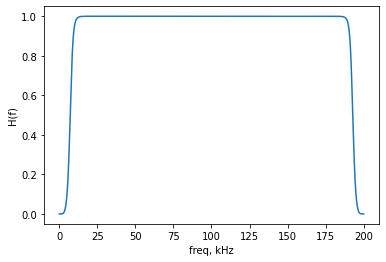
\includegraphics[width=0.5\textwidth]{./images/reponseEnFrequencePH8kHz.png}
\caption{Réponse fréquencielle du passe haut à 8kHz%
\label{fig:reponseEnFrequencePH8kHz}}
\end{figure}
Sur la réponse fréquencielle du filtre \ref{fig:reponseEnFrequencePH8kHz} on observe bien qu'au niveau de la fréquence de coupure qui est de 8kHz le signal est réduit de moitié.

Ainsi en appliquant simplement ce filtre on constate par exemple que l'identification du clic pour le zoom qui était impossible sans le filtre (à gauche sur \ref{fig:20000zoomavecetsansfiltrage}) sur le signal n° 20000 devient parfaitement possible avec (à droite sur \ref{fig:20000zoomavecetsansfiltrage}).

\begin{figure}[!h]
\centering
  \begin{subfigure}[b]{0.45\textwidth}
    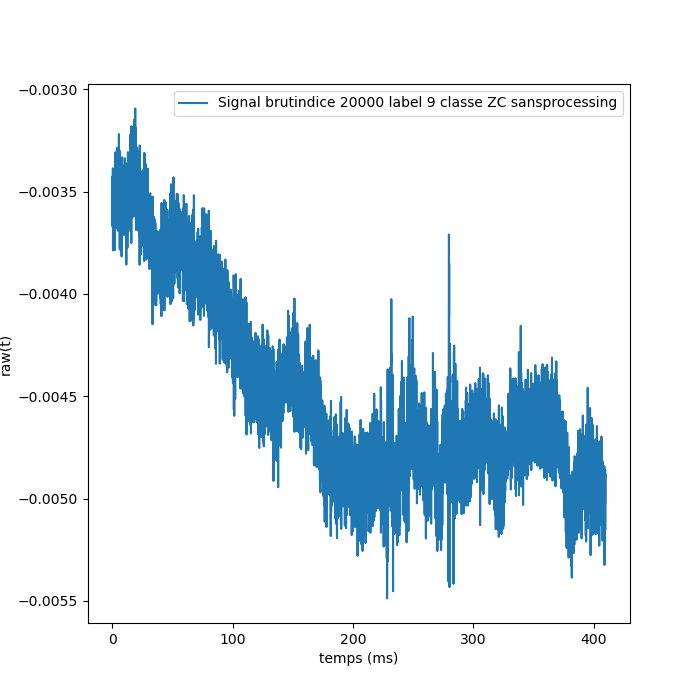
\includegraphics[width=\textwidth]{./images/indice20000Spectro1Dlabel9classeZCsansprocessingsanszoom.png}
    \caption{}
  \end{subfigure}
  \begin{subfigure}[b]{0.45\textwidth}
    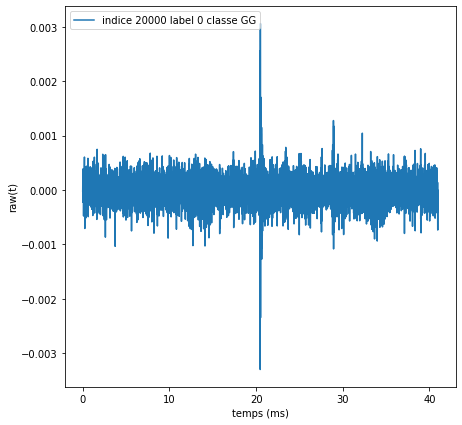
\includegraphics[width=\textwidth]{./images/indice20000Spectro1Dlabel9classeZCavecprocessingsanszoom.png}
    \caption{}
  \end{subfigure}
  \caption{Spectrogramme 3D des signaux : (a) n°20000 de la base d'apprentissage non filtré et (b) n°20000 de la base d'apprentissage filtré%
\label{fig:20000zoomavecetsansfiltrage}}
\end{figure}

\hypertarget{Mise-a-l-echelle}{%}
\subsection{Mise à l'échelle}
\label{Mise-a-l-echelle}}

En analysant les signaux, nous avons constaté de grandes différences aussi bien en terme d'intensité que de fréquences sur leurs clics.
Cependant, pour bien fonctionner le réseau de neurones convolutifs (comme la grande majorité des classifieurs) nécessite des données normalisées.
C'est pourquoi on va devoir mettre à l'échelle nos signaux, autrement dit nous allons normaliser automatiquement entre -1 et 1 l'ensemble de nos signaux.
Afin de réaliser celà on fait un choix pragmatique qui était de repérer le maximum puis diviser le signal par ce maximum.
Cette phase de normalisation se faisant après le filtrage passe haut des signaux,
il est raisonnable d'espèrer que la maximum du signal corresponde bien au clic.

\hypertarget{Les-Pipelines}{%}
\section{Les Pipelines}
\label{Les-Pipelines}}

A l'image des pipelines utilisés pour transporter le gaz ou le pétrole,
les pipelines en informatique servent à transporter un flux de données.
Flux de données sur lequel on va effectuer un certain nombre d'opérations, flux qui sera ensuite injecté  dans le réseau de neurones.
Cette méthode constitue maintenant la norme pour les applications en apprentissage automatique.

Elle présente plusieurs interêts majeurs :
\begin{itemize}
\item Elle évite d'avoir à stocker l'ensemble des résultats des opérations intermédiaires, permettant ainsi d'économiser beaucoup de mémoire.
\item Elle nous permet d'optimiser grandement l'ensemble du processus de prétraitement des données.
\item Elle favorise la réutilisation des procédures de traitement des données, par la normalisation dans leur définition.
\item Elle améliore grandement les performances lors de l'utilisation de frameworks disposant de fonctions adpatées pour les pipelines, comme TensorFlow, notamment pour l'implentation des traitements sur les cartes graphiques.
\end{itemize}

En pratique l'ensemble de nos fonctions étaient stockées dans un fichier python nommé cachalot\_helper, et à chaque essai on faisait passer notre flux de données par les fonctions désirées avant de l'injecter dans le réseau de neurones.


\hypertarget{Les-PDF}
\subsection{Génération des PDF}
\label{Guxe9nuxe9ration-des-PDF}}

Les bases de données contiennent un très grand nombre d'exemples (environ 130 000 au total que l'on peut visualiser sous 12 formes différentes soit potentiellement pls d'un million d'images).
Afin de pouvoir exploiter les analyses faites précédemment,  il a fallu développer un certain nombre d'outils afin de pouvoir aisement trier et manipuler les données.
Pour cela je me suis inspiré du systéme de pipeline que nous venons de voir, non pas pour
effectuer une tâche de classification, mais pour générer automatiquement des fiches d'analyse
des signaux.
L'avantage de cette méthode est que les fonctions de traitement utilisées pour l'apprentissage et pour la visualisation sont les mêmes, réduisant ainsi le risque d'erreurs lié aux doublons.

J'ai donc créé dans un script python définissant fonction paramètrable permettant tout d'abord de sélectionner un ou un plusieurs signaux dans un certain nombre de classes ou des signaux bien specifiques puis de générer automatiquement avec et ou sans preprocessing (les traitements du signal) avec ou sans zoom :
\begin{itemize}
\item Des courbes des signaux sélectionnés
\item Des spectrogrammes 2D des signaux sélectionnés
\item Des spectrogrammes 3D des signaux sélectionnés
\end{itemize}
Une fois générés, ils sont enregistrés sous forme de png dont le nom correspond à leur description. Ce qui donne par exemple pour le spectrogramme 3D sans processing et sans zoom de l'enregistrement numéro 17 000 de la classe GG dont le label est 0 :\\
indice17000Spectro3Dlabel0classeGGsansprocessingsanszoom.png.

A noter que les plots simples sont enregistrés sous spectro1D pour des raisons pratiques.

Dans un troisième temps, j'ai créé un autre script en python également paramètrable permettant de sélectionner des png en fonction de leur label, de leur type (spectrogramme 1D ou 2D ou 3D) et leurs options (avec ou sans zoom et avec ou sans processing).
Et de les intégrer dans un ou plusieurs fichiers latex en fonction de leur nombre.

Dans un quatrième temps, j'ai créé un autre script python, encore une fois paramètrable qui va récupérer les fichiers latex précedement créés, puis va les réunir dans un seul fichier latex.
Ce fichier latex est automatiquementcompilé par le script pour générer un fichier pdf
qui contient l'ensemble des courbes générées.
Ce fichier pdf est alors enregistré avec un nom correspondant à ce qu'il contient. Ainsi un fichier contenant les spectrogrammes 2D du label 6 sans processing et avec zoom sera nommé:\\ Spectro2Dlabel6sansprocessingaveczoom.pdf

Enfin un programme principal nommé apdfmaker, également paramètrable, est chargé de coordonner l'ensemble des scripts vus précedement.
A noter que ce programme ne se contente pas de générer un pdf à la fois mais peut
en générer une multitude à chaque exécution, en fonction des paramètres.
Ainsi si l'on veut par exemple qu'il génére toutes les représentations graphiques possibles (soit 1 080 000 images) de tous les enregistrements puis qu'il les stocke dans des pdf les plus détaillés possibles c'est théoriquement possible (même si cela n'est pas souhaitable  car très vite l'espace disque serait saturé).

Les pdf finaux ressemblerons à la figure~\ref{fig:exempledepdf}.

\begin{figure}[!h]
\centering
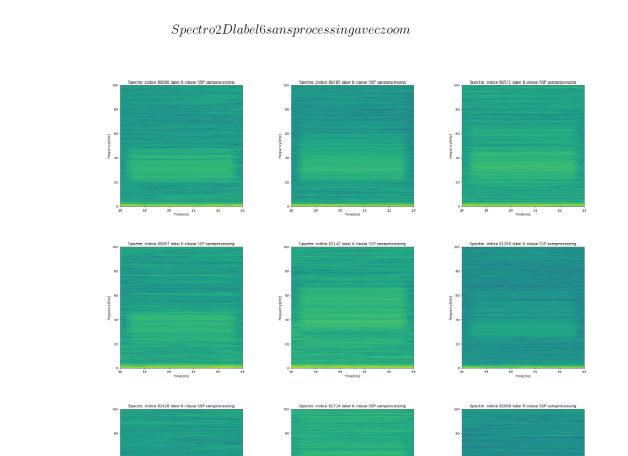
\includegraphics[width=10cm]{./images/pdfexemple.png}
\caption{Exemple de fiche d'analyse%
\label{fig:exempledepdf}}
\end{figure}
